\section{The Hash-and-Resubmit Pattern}

We now introduce a novel design pattern for Solidity smart contracts which
results into massive gas optimization due to the elimination of expensive
storage operations.

\textbf{Motivation.}
% This part is maybe too shallow. Consider deleting it. >>>> In the Ethereum
% blockchain, Turing-complete smart contracts were introduced. In order to
% prevent accidental or adversarial DoS phenomena such as infinite loops of
% code, contract invocations are bounded by an amount of gas units~\cite{wood,
% buterin}.  <<<<
It is essential for smart contracts to store data in the blockchain. However,
interacting with the storage of a contract is among the most expensive
operations of the EVM. Therefore, only necessary data should be stored and
redundancy should be avoided when possible. This is contrary to conventional
software architecture, where storage is considered cheap. Usually, the
performance of data access in traditional systems is related with time.
However, in Ethereum performance is related to gas consumption. Access to
persistent data costs a substantial amount of gas, which has a direct monetary
value. One way to mitigate gas cost of reading variables from the blockchain is
to declare them public.  This leads to the creation of a \emph{getter} function
in the background, allowing free access to the value of the variable. But this
treatment does not prevent the initial population of storage data, which is
significantly costly, especially for large size of data. Towards the goal of
implementing gas-efficient smart contracts, several patterns have been
proposed~\cite{contract-opt-1, contract-opt-2, contract-opt-3}.

By using the \emph{hash-and-resubmit} pattern, large storage variables are
omitted entirety, and structures are contained in memory which results to
vastly improved performance. When a function call is performed, the arguments
and signature of the function is included in the transactions field of the body
of a block. The contents of blocks are public to the network, therefore this
information is available to nodes. By simply observing blocks, a node retrieves
data sent by other users, which be processed off-chain. To advertise the
process of data to the public network, the node re-sends the retrieved data
accompanied with complementary data depending on the context of the
application. While the concept of resending data would be inefficient in
conventional systems \[...\]
% the cost of addressing memory is  storage is   in Solidity

\noindent
\textbf{Applicability.}
We now list the cases in which the \emph{hash-and-resubmit} pattern is
efficient to use:
\begin{enumerate}
    \item Avoid high gas cost due to extensive storage read/write and make
        smart contracts that exceed block gas limit practical.
    \item Interact with smart contract depending of previous actions of
        other users
    \item Process data off-chain
\end{enumerate}

\newcommand{\contract}{\mathsf{S}}
\newcommand{\client}{\mathsf{E_{1}}}
\newcommand{\observer}{\mathsf{E_{2}}}
\newcommand{\data}{\mathsf{d}}
\newcommand{\datao}{\mathsf{d^*}}

\noindent \textbf{Participants and collaborators.} The participants are the
smart contract $\contract$ which accepts function calls, the client $\client$,
who dispatches arbitrary data $\data$ to $contract$ \texttt{send($\data$)}, and
the observer $\observer$, who is a node that observes transactions towards
$\contract$ in the blockchain. After observation, $\observer$ retrieves data
$\data$. Finally, $\observer$ acts as a client, making an interaction with
$\contract$, \texttt{send($\data$)}. However, we need to consider that since
the retrieval was realized off-chain, a malicious $\observer$ may alter $\data$
before interacting with $\contract$. We will denote the potentially modified
data as $\datao$. The verification that $\data = \datao$ consists a part of the
pattern and is performed during \texttt{send($\datao$)}.

\noindent \textbf{Implementation.} The implementation of this pattern is
divided into two parts. The first part covers the way $\datao$ is retrieved by
$\observer$, whereas the second part explains how the we verify that
$\data=\datao$. The challenge here is twofold:

\begin{enumerate}

    \item Availability: $\observer$ must be able to retrieve $\data$ without
        the need of accessing on-chain data.

    \item Consistency: $\observer$ must be prevented from dispatching $\datao$
        that differs from the originally submitted $\data$.

\end{enumerate}

\noindent
\emph{Hash-and-resubmit} technique is performed in two
stages to face these challenges: (a) the \emph{hash} phase, which addresses
\emph{reliability}, and (b) the \emph{resubmit} phase which addresses
\emph{availability}.

\noindent \textsf{Addressing availability:} During \emph{hash} phase, $\client$
makes the function call \texttt{send($\data$)}. This transaction, which
includes a function signature (\texttt{send}) and the corresponding data
($\data$), is added in a block by a miner.  Due to blockchain's transparency,
the observer of \texttt{send}, $\observer$, retrieves a copy of $\data$,
without the need of accessing contract data.

\noindent \textsf{Addressing reliability:} We prevent an adversary $\observer$
from altering $\datao$ by storing the \emph{hash} of $\data$ in contract's
state during the execution of \texttt{send($\data$)} by $\client$. Although we
can make use of any cryptographic hash function it is convenient to use the
pre-compiled \texttt{sha256} hash function of Solidity: \[hash =
\texttt{sha256}(\data)\] Then, during contest phase, a verification is
performed by comparing the stored hash of $\data$ with the hash of $\datao$.
\[\texttt{require}(hash = \texttt{sha256}(datao)\]
\noindent In solidity, the
size of the hash is 32 bytes. To persist such a small value in contract's
memory only adds a constant, negligible cost overhead.

\noindent \textbf{Sample.} We will now demonstrate the usage of the
hash-and-resubmit pattern with a practical example. We create a smart contract
that orchestrates a game between two players, $P1$ and $P2$. The winner is the
player with the most valuable array. The interaction between the players and
the smart contract is realized in two phases: (a) Submit phase and (b) Contest
phase.

\noindent \textsf{Submit phase:} $P1$ submits an N-sized array, $array_1$ and
becomes the $holder$ of the contract.

\noindent \textsf{Contest phase:} $P2$ submits $array_2$. If $array_2$ $>$
$array_1$, then the $holder$ of the contract is changed. The comparison between
the two arrays can be implemented arbitrarily.

We make use of the \emph{hash-and-resubmit} pattern by demanding from $P2$ to
provide \emph{two} arrays to the contract during contest phase: (a)
$array_1^*$, which is a copy of the originally submitted array by $P1$, and (b)
$array_2$, which is the contesting array.

We show the storage implementation of the above game in
Algorithm~\ref{alg.compare-storage} and the hash-and-resubmit version in
Algorithm~\ref{alg.compare-memory}.

\begin{algorithm}
    \label{alg.compare-storage}
    \caption{\textsf{Compare} N-sized arrays using storage}
    \begin{algorithmic}[1]
        \Function{\sf Submit}{$array$}
            \State $best\_array \gets array$
            \Comment{array saved in storage}
            \State $holder \gets msg.sender$
            \State\Return{true}
        \EndFunction
    \vskip8pt
    \end{algorithmic}

    \begin{algorithmic}[1]
        \Function{\sf Contest}{$new\_array$}
        \If{!compare($new\_array$)}
            \State\Return{false}
        \EndIf
        \State $holder \gets msg.sender$
        \State\Return{true}
    \EndFunction
    \vskip8pt
    \end{algorithmic}

    \begin{algorithmic}[1]
        \Function{\sf compare}{$new\_array$}
            \For{$i$ in $best\_array$.length}
            \If{$new\_array$[$i$] $\leq$ $best\_array$[$i$]}
                    \State\Return{false}
                \EndIf
            \EndFor
            \State\Return{true}
        \EndFunction
        \vskip8pt
    \end{algorithmic}
\end{algorithm}

\begin{algorithm}
    \label{alg.compare-memory}
    \caption{\textsf{Compare} N-sized arrays using hash-and-resubmit pattern}
    \begin{algorithmic}[1]
        \Function{\sf Submit}{$array[N]$}
        \State $hash \gets sha256(array)$
            \Comment{hash saved in storage}
            \State $holder \gets msg.sender$
            \State\Return{true}
        \EndFunction
    \vskip8pt
    \end{algorithmic}

    \begin{algorithmic}[1]
    \Function{\sf Contest}{$existing\_array$, $new\_array$}
    \If{hash256($existing\_array$) $\neq$ $hash$}
        \State\Return{false}
        \Comment{Invalid $original\_array$}
    \EndIf

    \If{!compare($original\_array$, $new\_array$)}
        \State\Return{false}
    \EndIf
    \State $holder \gets msg.sender$
    \State\Return{true}
    \EndFunction
    \vskip8pt
    \end{algorithmic}

    \begin{algorithmic}[1]
        \Function{\sf compare}{$array_1$, $array_2$}
            \For{$i$ in $array_1$.length}
                \If{$array_1$[$i$] $\leq$ $array_2$[$i$]}
                    \State\Return{false}
                \EndIf
            \EndFor
            \State\Return{true}
        \EndFunction
        \vskip8pt
    \end{algorithmic}
\end{algorithm}


\noindent \textbf{Gas analysis.} The gas consumption of the two
algorithms is displayed in Figure~\ref{fig:har-example}.

\begin{figure}[h!]
\begin{center}
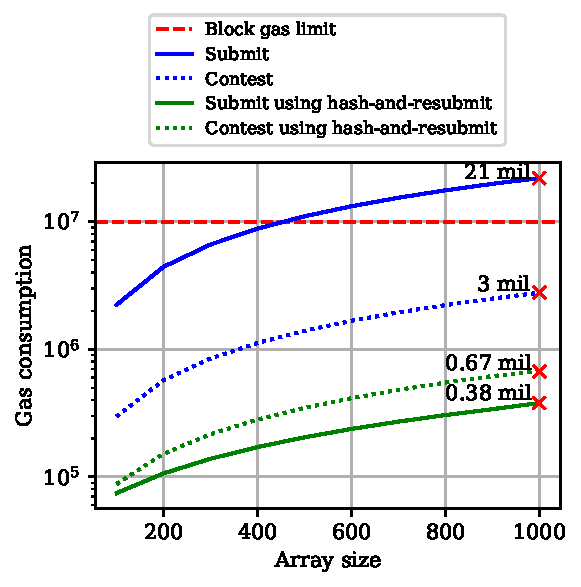
\includegraphics[width=1 \columnwidth]{figures/har-example.pdf}
\end{center}
\caption{Gas-cost reduction using the \emph{hash-and-resubmit} pattern. By
avoiding gas-heavy storage operations, the cost of function invocations is
decreased significantly by 93-95\%.}
\label{fig:har-example}
\end{figure}

By using the \emph{hash-and-resubmit} pattern, the gas consumption decreased by
93-95\%. This significantly affects the applicability of the contract. Note
that, the storage implementation exceeds the Ethereum block gas
limit\footnote{As of July 2020, the Ethereum block gas limit approximates
10,000,000 gas units} for arrays of size 500 and above, contrary to the
hash-and-resubmit-optimized version, which consumes approximately 1/10th of the
block gas limit for arrays of 1000 elements.

\noindent
\textbf{Consequences}

\noindent \textbf{Known uses.} To our knowledge, we are the first to combine
the notion of the transparency of the blockchain with signatures of data
structures to eliminate storage variables from Solidity smart contracts by
resubmitting data.

\noindent \textbf{Hash-and-Resubmit.} We introduce a novel design pattern for
Solidity smart contracts that results into massive gas optimization. This
technique, which we term \emph{hash-and-resubmit}, is based on observing public
data of the blockchain in order to leverage \emph{off-chain} operations. By
utilizing \emph{hash-and-resubmit}, the performance of the smart contract is
improved considerably since computations are performed locally by the user, and
gas-heavy storage variables are discarded.

The critical observation we make is that persistent data structures, i.e.
arrays, can be migrated from storage to memory space. Such an adjustment
results to substantial increase of smart contracts' performance due to the
sizable discrepancy between persistent and temporary memory operations.

This is due to the fact that in the body of
the Ethereum block, information regarding transactions is stored. Nodes have
access to this information which includes signatures and input arguments of
function invocations, as shown in Figure~\ref{fig:observe-tx}. This type of
\emph{off-chain} access can be applied by any node.

\begin{figure}[h]
    \begin{center}
        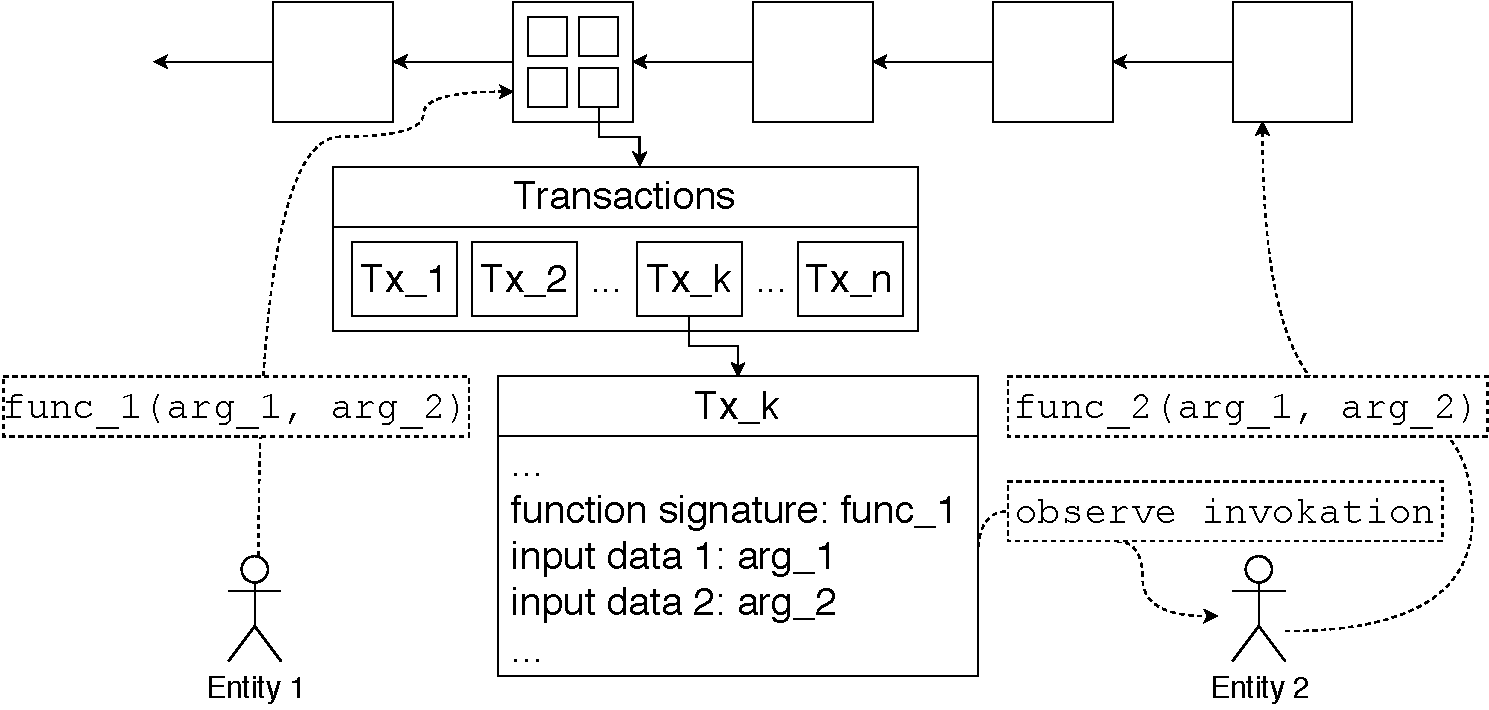
\includegraphics[width=1\columnwidth]{figures/observer-tx.pdf}
    \end{center}
    \caption{Entity 1 makes a function call with arguments arg1 and arg2.
    Entity 2 reads the content of transactions in the block and retrieves the
    input data. Entity 2 can use this data to make a different invocation.}
    \label{fig:observe-tx}
\end{figure}

\noindent \textbf{Enabling NIPoPoWs.} We now present how the
\emph{hash-and-resubmit} pattern can used in the context of the NIPoPoW
superlight client. Similar to the aforementioned example, the NIPoPoW verifier
adheres to a submit-and-contest-phase schema, and the inputs of the functions
are arrays that are processed on-chain.

In \emph{submit-phase}, a \emph{proof} is submitted, which can be contested by
another user in \emph{contest-phase}.  The user that initiates the contest,
needs to monitor the traffic of the smart contract. This is a logical
assumption as mentioned in the NIPoPoW paper. The input of \texttt{submit}
function includes the \emph{submit proof}, $\pi_{subm}$, that indicates the
occurrence of an \emph{event}, $e$, in the source chain, and the input of
\texttt{contest} function includes the \emph{contesting proof}, $\pi_{cont}$. A
successful contest of the $\pi_{subm}$ is realized when $\pi_{cont}$ a
better score. The process of score evaluation, which is described in
~\cite{nipopows} is irrelevant to the pattern, and remains unchained.

In previous work~\cite{gglou}, NIPoPoW arrays are stored on-chain during
submit-phase, and are processed during contest-phase. This operation is
performed by utilizing storage, which limits the applicability of the contract
considerably. In Algorithm~\ref{alg:har-nipopow} we show how hash-and-resubmit
pattern is embedded into the NIPoPoW client. In Figure~\ref{fig:har-nipopow} we
display how the gas consumption differentiates from previous work for the
aggregated cost of submit and contest phase.


\newcommand{\genesis}{\textsf{G}}

\begin{algorithm}
    \label{alg:har-nipopow}
    \caption{The \textsf{NIPoPoW} client using hash-and-resubmit pattern}
    \begin{algorithmic}[1]

    \Contract{crosschain}
    \State $\textsf{events} \gets \bot;$ $\genesis \gets \bot$
    \Function{\sf initialize}{$\genesis_{remote}$}
        \State \genesis $\gets \genesis_{remote}$
    \EndFunction
    \Function{\sf submit}{$\pis$, $e$}
        \State \textsf{require}($\pis$[0] = $\genesis$)
        \State \textsf{require}($\textsf{events$[e]$} = \bot$)
        \State \textsf{require}($\textsf{valid-interlink}(\pi)$)
        \State \textsf{DAG} $\gets$ \textsf{DAG} $\cup$ $\pis$
        \State \textsf{events$[e]$.hash} $\gets$ \textsf{H}($\pis$)
        \Comment{enable pattern}
        \State \textsf{ancestors} $\gets$ \textsf{find-ancestors()}
        \State \textsf{events$[e]$.pred} $\gets$
            \textsf{evaluate-predicate}(\textsf{ancestors}, e)
        \State \textsf{ancestors} $=$ $\bot$
    \EndFunction
    \Function{\sf contest}{$\pisa$, $\pic$, $e$}
        \Comment{provide proofs}
        \State \textsf{require}(\textsf{events$[e]$.hash} $=$ \textsf{H}($\pisa$))
        \Comment{verify $\pisa$}
        \State \textsf{require}($\pic$[0] = $\genesis$)
        \State \textsf{require}(\textsf{events}$[e]$ $\ne$ $\bot$)
        \State \textsf{require}(\textsf{valid-interlink}($\pi_{cont}$))
        \State $lca$ = \textsf{find-lca}($\pisa$, $\pic$)
        \State \textsf{require}(\textsf{score}($\pic[:lca]$)
            $>$ \textsf{score}($\pisa[:lca]$))
        \State \textsf{DAG} $\gets$ \textsf{DAG} $\cup$ $\pic$
        \State \textsf{ancestors} $\gets$ \textsf{find-ancestors}(\textsf{DAG})
        \State \textsf{events$[e]$.pred} $\gets$
            \textsf{evaluate-predicate}(\textsf{ancestors}, $e$)
        \State \textsf{ancestors} $=$ $\bot$
    \EndFunction
    \EndContract
    \vskip8pt
    \end{algorithmic}
\end{algorithm}



\begin{figure}[h]
    \begin{center}
        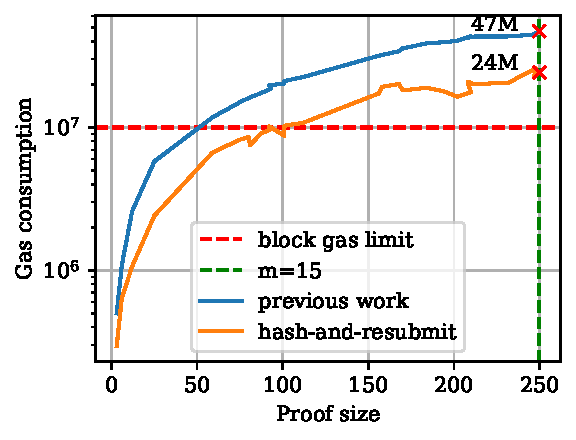
\includegraphics[width=1\columnwidth]{figures/har-nipopows.pdf}
    \end{center}
    \caption{Performance improvement using hash-and-resubmit pattern in
    NIPoPoWs related to previous work. The gas consumption decreased by
    approximately 50\%}
    \label{fig:har-nipopow}
\end{figure}
